
\clearpage
\begin{figure}
\includegraphics[width=\textwidth]{hipparcos2_properties.ps}
\caption{Properties of the kinematically unbiased subsample of main-sequence stars extracted from the \Hipparcos\ catalogue. The diagonal shows histograms of the relative abundances of stars in the basic properties right ascension (\ra), declination (\dec), parallax ($\pi$), proper motion in \ra\ (\pmrastar), which includes a factor of $\cos \dec$, and proper motion in \dec\ (\pmdec). The plots in the upper-right triangle show two-dimensional scatter plots of pairs of these properties, while the lower-left triangle shows two-dimensional histograms for these pairs.}%
\label{fig:hip2prop}%
\end{figure}

\clearpage
\begin{figure}
\includegraphics{veldensXY.ps}
\caption{Projection on the $v_x-v_y$ plane of the reconstructed velocity distribution as a function of the number of Gaussians $K$ and the regularization parameter $w$ used in the reconstruction. The density grayscale is linear and contours contain, from the inside outward, 2, 6, 12, 21, 33, 50, 68, 80, 90, 95, 99, and 99.9 percent of the distribution. The first five of these contours are white and somewhat blended together in some of the panels; 50 percent of the distribution is contained within the innermost dark contour. The origin in each of these plots is at the Solar velocity.}%
\label{fig:veldensXY}
\end{figure}


\clearpage
\begin{figure}
\includegraphics{veldensXZ.ps}
\caption{Same as Fig.~\ref{fig:veldensXY}, but projected onto the $v_x-v_z$ plane.}%
\label{fig:veldensXZ}
\end{figure}


\clearpage
\begin{figure}
\includegraphics{veldensYZ.ps}
\caption{Same as Fig.~\ref{fig:veldensXY}, but projected onto the $v_y-v_z$ plane.}%
\label{fig:veldensYZ}
\end{figure}


\clearpage
\begin{figure}
\includegraphics{loglike.ps}
\caption{Likelihood of the reconstructed velocity distribution given the tangential velocities of the \Hipparcos\ stars as a function of the number of Gaussians $K$ and the regularization parameter $w$ used in the reconstruction. The likelihood increases as the number of Gaussians is increased and as the regularization parameter is decreased. The white cross indicates the position of the maximum.}%
\label{fig:loglike}
\end{figure}


\clearpage
\includegraphics{predict_gcs_rand.ps}
\clearpage
\begin{figure}
\caption{Predicted radial velocity distribution using the reconstructed velocity distribution with $k$ = 10, $w$ = 4 km$^2$ s$^{-1}$ for random stars in the \gcsabb\ catalogue. The gray curve gives the radial velocity distribution obtained by marginalizing the three-dimensional velocity distribution over the tangential velocity (see \eqnnumber~[\ref{eq:margpredicted}]), while the black curve shows the radial velocity distribution obtained by conditioning the reconstructed velocity distribution on the tangential velocity of the star as measured by \Hipparcos (see \eqnnumber~[\ref{eq:condpredicted}]). The black vertical line gives the measured value of the radial velocity from the \gcsabb\ catalogue. The gray vertical lines give the 95-percent confidence interval limits for the conditional distribution. The entropies $H_1$ and $H_2$ of the conditional, respectively marginalized distribution are given in the upper-right corner. The \Hipparcos\ number of the star is given in the upper-left corner.}%
\label{fig:predict_gcs_rand}
\end{figure}

\clearpage
\begin{figure}
\includegraphics{tile_onepred.ps}
\caption{Predicted radial velocity distribution using the reconstructed velocity distribution as a function of the number of Gaussians $K$ used in the reconstruction and the regularization parameter $w$ for a random star in the \gcsabb\ catalogue (the star with \Hipparcos\ number HIP50568). See Fig.~\ref{fig:predict_gcs_rand} for an explanation of the different lines in each panel.}%
\label{fig:tile_onepred}
\end{figure}


\clearpage
\begin{figure}
\includegraphics[width=.315\textwidth]{crossval.ps}\hfill
\includegraphics[width=.315\textwidth]{aic.ps}\hfill
\includegraphics[width=.315\textwidth]{mdl.ps}\\[10pt]
\includegraphics[width=.315\textwidth]{mml.ps}\hfill
\includegraphics[width=.315\textwidth]{bayes.ps}\hfill
\includegraphics[width=.315\textwidth]{gcs_cross.ps}
\caption{Model selection surfaces: These surfaces show the different model selection criteria defined in the text applied to the reconstruction of the velocity distribution from \Hipparcos\ data. Models are defined by the number of Gaussian components $K$ and a regularization parameter $w$. In each of these figures a darker color represents a model that is more favored by the model selection criterium at hand; the white cross indicates the most favored model for each model selection criterium. Shown are (from left to right and from top to bottom): (1) cross-validation; (2) Akaike's Information Criterion (\AIC); (3) Minimum Description Length (\MDL); (4) Minimum Message Length (\MML); (5) Bayesian evidence; and (6) the likelihood of the predicted radial velocity distribution using radial velocities from the \gcsabb\ catalogue.}%
\label{fig:modelselection}
\end{figure}


\clearpage
\begin{figure}
\includegraphics{checkquants.ps}
\caption{Distribution of the quantile of the predicted radial velocity distribution (using $K$ = 10 and $w$= 4 km$^2$ s$^{-2}$) at which the radial velocity from the \gcsabb\ catalogue is found for all the stars from the sample we selected from the \gcsabb\ catalogue. If the probability distribution of the radial velocity for each star was entirely correct this curve should be flat at $P(f) = 1$.}%
\label{fig:checkquants}
\end{figure}

\clearpage
\begin{figure}
\includegraphics{predict_gcs_good.ps}
\caption{The six ``best'', \ie, highest likelihood, predictions of the radial velocity of stars in the \gcsabb\ catalogue based on our reconstruction of the velocity distribution with $K$ = 10 and $w$= 4 km$^2$ s$^{-2}$.}%
\label{fig:predict_gcs_good}
\end{figure}

\clearpage
\begin{figure}
\includegraphics{predict_gcs_bad.ps}
\caption{Same as Fig.~\ref{fig:predict_gcs_good}, but the six ``worst'', \ie, lowest likelihood, predictions.}%
\label{fig:predict_gcs_bad}
\end{figure}

\clearpage
\begin{figure}
\includegraphics{hist_gcs_like.ps}
\caption{Top: distribution of the likelihood of the predicted radial velocity distribution (with $K$ = 10 and $w$ = 4 km$^2$ s$^{-2}$) given stars from the \gcsabb\ catalogue. Bottom: two-dimensional histogram of the radial velocities from the \gcsabb\ catalogue and their probability under the reconstructed velocity distribution (gray scales are logarithmical).}%
\label{fig:hist_gcs_like}
\end{figure}

\clearpage
\begin{figure}
\includegraphics{predict_gcs_low.ps}
\caption{The six ``tightest'', \ie, lowest entropy, predictions of the radial velocity of stars in the \gcsabb\ catalogue based on our reconstruction of the velocity distribution with $K$ = 10 and $w$= 4 km$^2$ s$^{-2}$.}%
\label{fig:predict_gcs_low}
\end{figure}

\clearpage
\begin{figure}
\includegraphics{predict_gcs_high.ps}
\caption{Same as Fig.~\ref{fig:predict_gcs_low}, but the six ``widest'', \ie, highest entropy, predictions.}%
\label{fig:predict_gcs_high}
\end{figure}


\clearpage
\begin{figure}
\includegraphics{hist_gcs_ent.ps}
\caption{Top: distribution of the entropy of the predicted radial velocity distribution (with $K$ = 10 and $w$ = 4 km$^2$ s$^{-2}$) for stars from the \gcsabb\ catalogue. Bottom: two-dimensional histogram of the likelihood of the predicted radial velocity distributions given stars from the \gcsabb\ catalogue and the entropy of the predicted distribution (gray scales are logarithmical).}%
\label{fig:hist_gcs_ent}
\end{figure}



\clearpage
\begin{figure}
\includegraphics{radecpatches.ps}
\caption{Predicted radial velocity distribution for stars in different directions on the celestial sphere and observed distribution from the \gcsabb\ catalogue for different (\ra,\dec)-patches on the sky. Stars are selected to lie within 20$\degree$ of the central \ra\ and within 10$\degree$ of the central \dec, or in the corresponding region around the opposite \ra\ and \dec. The predicted radial velocity distribution is calculated by marginalizing the reconstructed velocity distribution using $K$= 10 and $w$ = 4 km$^2$ s$^{-2}$ at the center of each patch. The central \ra\ and \dec\ are given in the upper-right corner of each panel. The number of stars in the \gcsabb\ sample in the relevant (\ra,\dec)-patch are given in the upper-left corner of each panel.}%
\label{fig:radecpatches}
\end{figure}


\clearpage
\begin{figure}
\includegraphics{info_hip_low.ps}
\caption{The six ``tightest'', \ie, lowest entropy, predictions of the radial velocity of stars in the sample we extracted from the \Hipparcos\ catalogue that do not have an entry in the \gcsabb\ catalogue based on our reconstruction of the velocity distribution with $K$ = 10 and $w$= 4 km$^2$ s$^{-2}$.}%
\label{fig:info_hip_low}
\end{figure}

\clearpage
\begin{figure}
\includegraphics{info_hip_high.ps}
\caption{Same as Fig.~\ref{fig:info_hip_low}, but the six ``widest'', \ie, highest entropy, predictions.}%
\label{fig:info_hip_high}
\end{figure}


\clearpage
\begin{figure}
\includegraphics{hist_hip_ent.ps}
\caption{Distribution of the entropy of the predicted radial velocity distribution (with $K$ = 10 and $w$ = 4 km$^2$ s$^{-2}$) for stars in the sample we extracted from the \Hipparcos\ catalogue that do not have an entry in the \gcsabb\ catalogue.}%
\label{fig:hist_hip_ent}
\end{figure}


\clearpage
\begin{figure}
\includegraphics[width=\textwidth]{annotated_veldist.ps}
\caption{Two-dimensional projections of the reconstructed velocity distribution with $K$ = 10 Gaussians and $w$ = 4 km$^2$ s$^{-2}$. Contours are as in \figurename~\ref{fig:veldensXY}. The origin is at the Solar velocity and the velocity of the Local Standard of Rest \citep{2005ApJ...629..268H} is indicated by a triangle.}%
\label{fig:annotated_veldist}
\end{figure}

\clearpage
\begin{figure}
\includegraphics[height=0.717\textheight]{annotated_veldist2.ps}
\caption{Projection of the reconstructed velocity distribution with $K$ = 10 Gaussians and $w$ = 4 km$^2$ s$^{-2}$ in the $\vx$--$\vy$ plane: Velocity distribution with the moving groups indicated (\emph{top panel}); 1--sigma covariance ellipses around the mean of each Gaussian component $j$ with a linewidth proportional to the natural logarithm of its amplitude $\alpha_j$ (\emph{bottom panel}). Contours in the top panel are as in \figurename~\ref{fig:veldensXY}, but without the 99 and 99.9\,percent contours. The origin is at the Solar velocity and the velocity of the Local Standard of Rest \citep{2005ApJ...629..268H} is indicated by a triangle.}%
\label{fig:annotated_veldist2}
\end{figure}



\end{document}
